This section outlines the timeline for the project, including the various phases, key milestones, and the overall schedule depicted in the Gantt chart. The timeline is designed to ensure the project progresses smoothly and all deliverables are met within the specified timeframe.

\vspace{12pt}
\subsection{Project Phases}
\vspace{12pt}

The key project phases are structured to guide the project from initiation to completion. Each phase has specific objectives and tasks that contribute to the successful delivery of the project. The phases are:
\begin{enumerate}
    \item Project Initiation: Conducting the Literature Review, Defining the project scope, objectives, and deliverables.
    \item Tool Selection and Setup: Identifying and configuring the necessary tools and technologies.
    \item Implementation: Developing and integrating the project components.
    \item Evaluation: Testing and validating the project's outcomes.
    \item Documentation and Presentation: Preparing the final documentation and presenting the project results.
\end{enumerate}

\vspace{12pt}
\subsection{Milestones}
\vspace{12pt}

To monitor progress and ensure timely completion, the project includes several key milestones. These milestones mark significant points in the project and serve as checkpoints to review progress. The milestones are:
\begin{enumerate}
    \item Literature Review Completion: Completing the review of relevant literature and research.
    \item Project Proposal Submission: Submitting the detailed project proposal.
    \item First Prototype: Developing and testing the initial prototype.
    \item Final Solution: Completing the final version of the project.
    \item Research Paper Submission: Submitting the research paper detailing the project outcomes.
    \item Final Report Submission: Submitting the comprehensive final report of the project.
\end{enumerate}

\vspace{12pt}
\subsection{Gantt Chart}
\vspace{12pt}

The following Gantt chart conveys the estimated timeline, project deliverables, and the planned stages of the project. It provides a visual representation of the project schedule and helps in tracking the progress of each phase and milestone.

\begin{figure}[htbp]
  \centering
  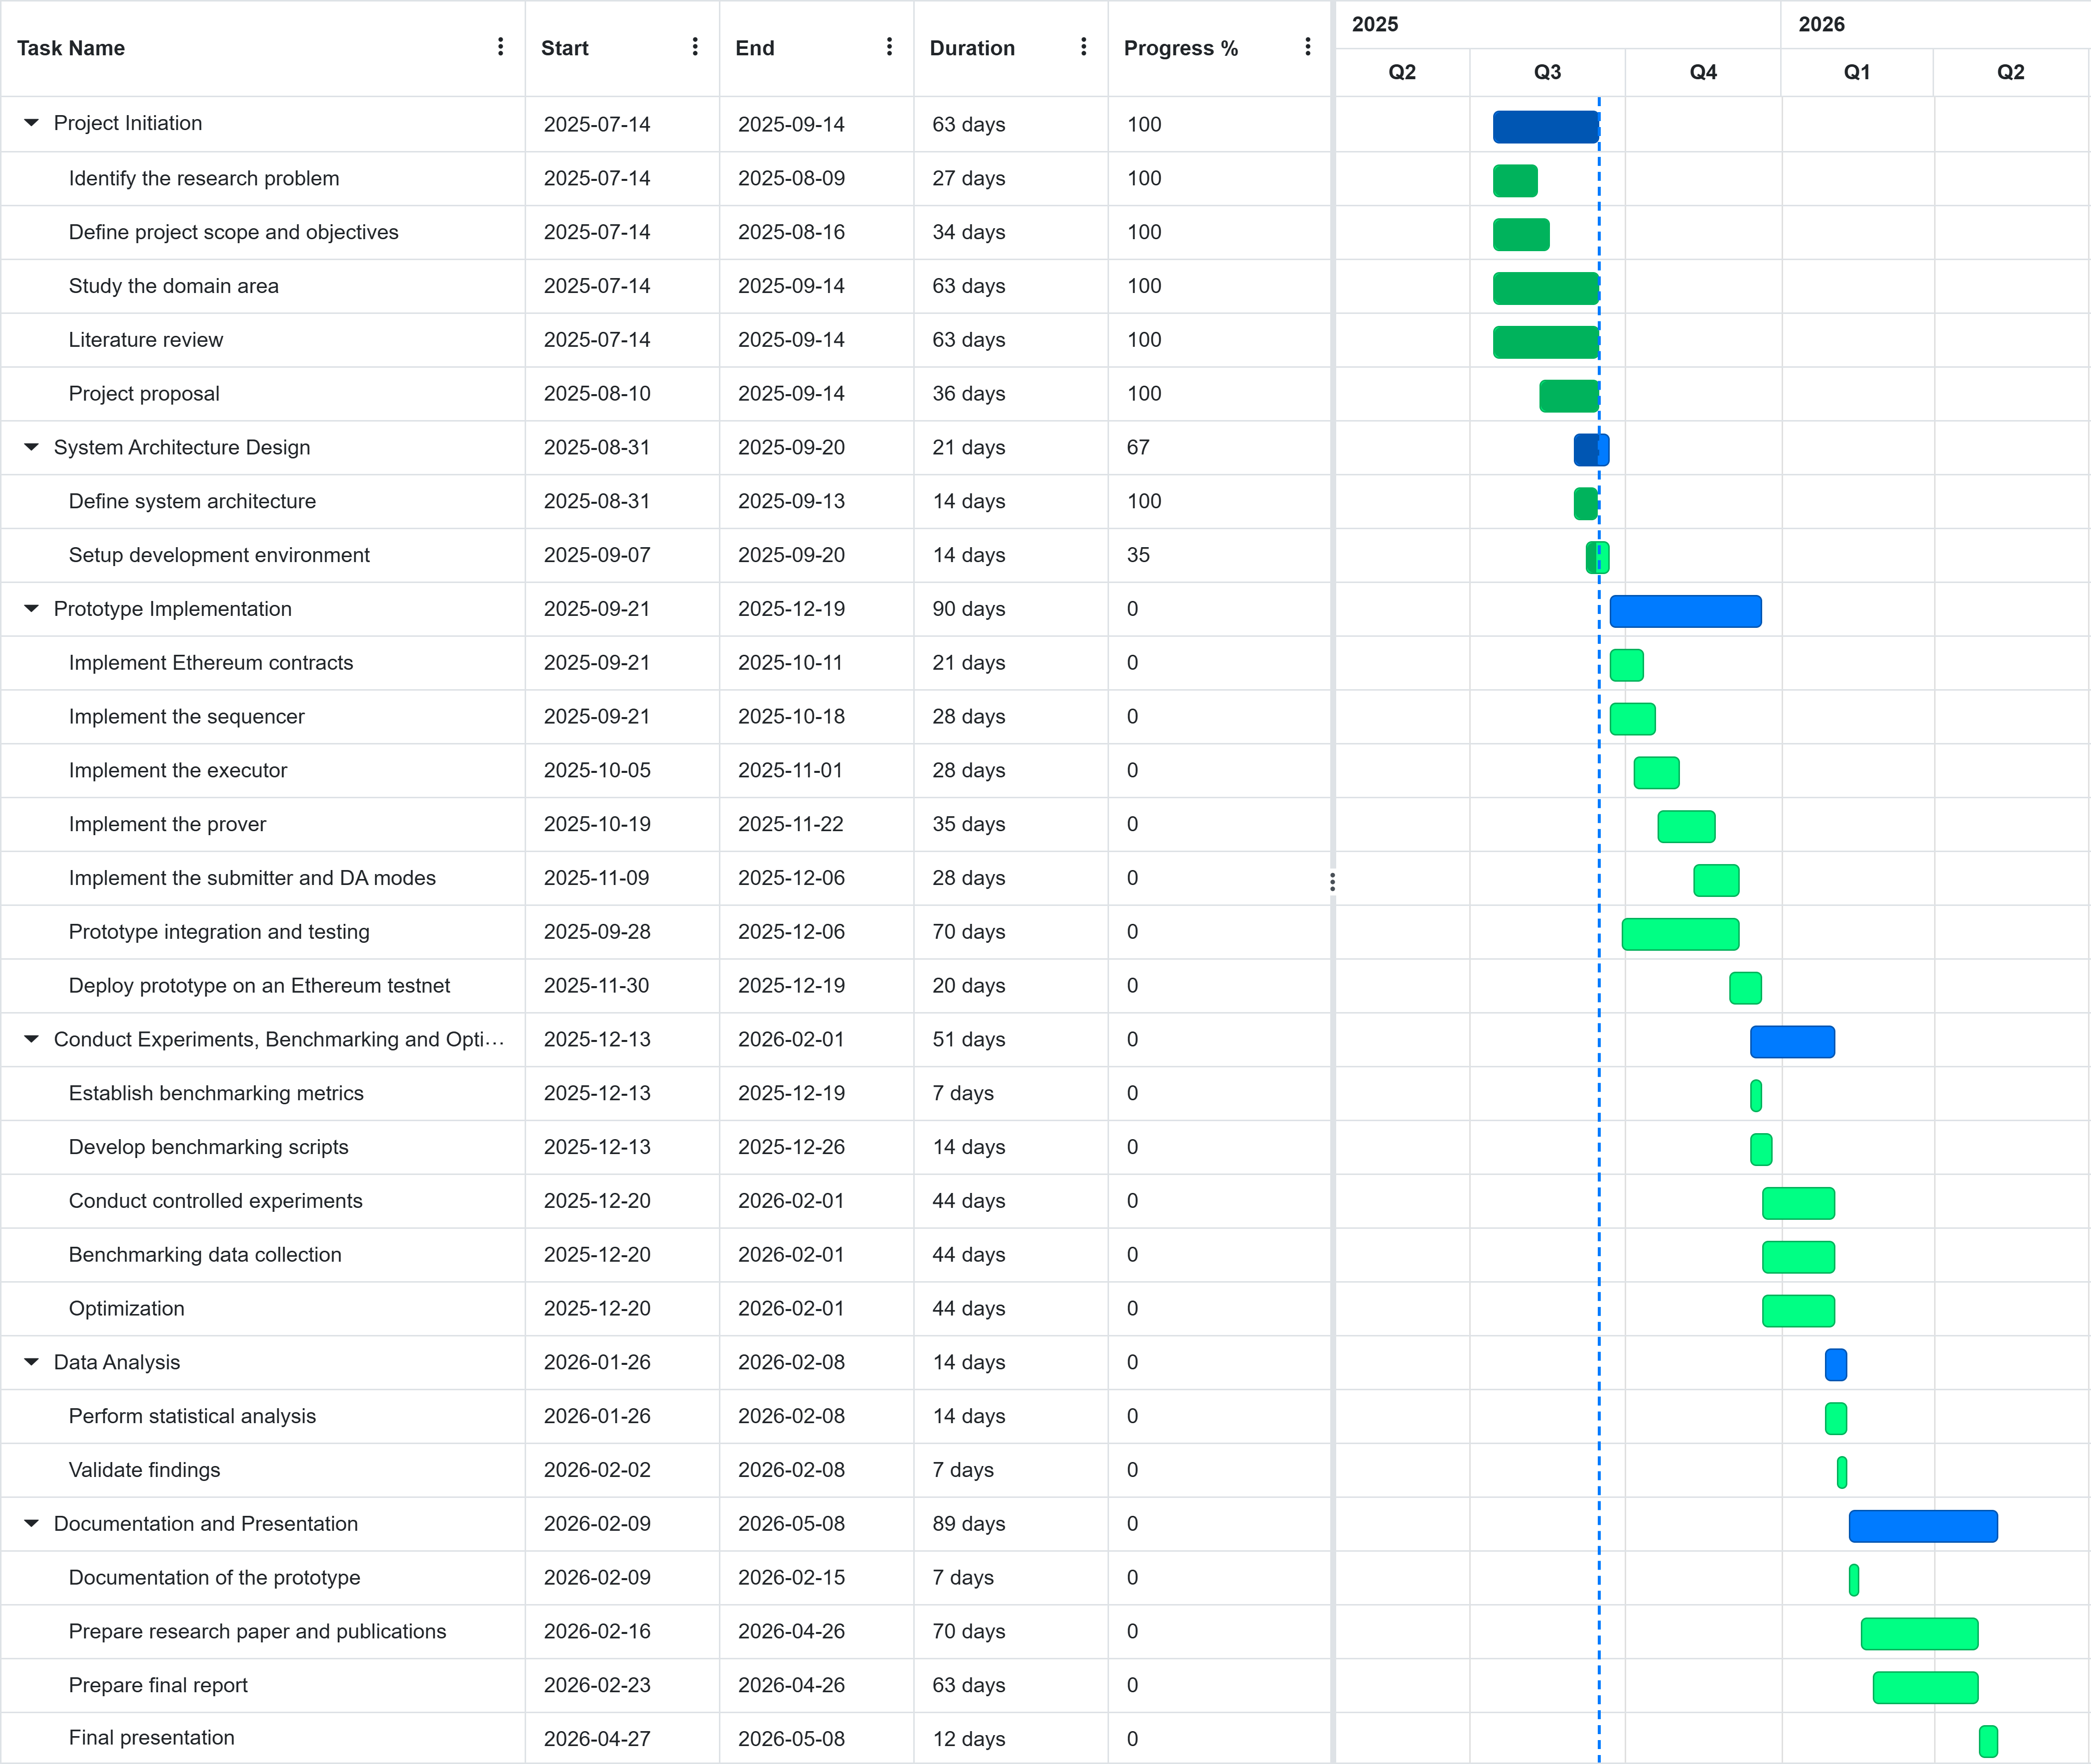
\includegraphics[height=0.8\linewidth, angle=90]{figures/proposed-timeline.png}
  \caption{Gantt Chart for the project timeline}
  \label{fig:operation-flow}
\end{figure}


\clearpage